
\documentclass[12pt]{article}
\usepackage{amsmath}

\usepackage{indentfirst}
\usepackage[font=scriptsize]{caption}
%\usepackage[font=small]{caption}10
%\usepackage[font=footnotesize]{caption}%9
%\usepackage[font=scriptsize]{caption}%8

\usepackage[utf8]{inputenc}
\usepackage{graphicx}
\usepackage{hyperref}
\usepackage[letterpaper,margin=0.75in]{geometry}
\usepackage{setspace}
\usepackage{comment}
\usepackage{amsmath}
\usepackage{esint}
\usepackage{wrapfig}
\usepackage{lipsum}
\usepackage{subcaption}
\usepackage{caption}

\begin{document}

\doublespacing


\begin{center}
{\Large \textbf{Developments of a Simple Model to Elucidate the Shape of Enveloped Viruses: Motivated by Monkeypox and SARS-CoV-2}}\\[1.5ex]
{\normalsize  Hua Deng}\\

{\normalsize February 21, 2025}
\end{center}





\begin{flushleft}
\setlength{\parindent}{30pt}
\section*{Specific aim}
First, to develop new models and simulations to study how the viral genome architecture(its shape, length and flexibility) influences the membrane. By combining polymer physics and liquid-state physics, such as crowding effects, we hope to gain a deeper understanding of viral assembly. By simulating how viral genomes behave in confined environments, we can uncover key principles behind virus formation and stability. It could contribute to more effective strategies for prevention and treatment of viral infections, especially for viruses like Monkeypox and SARS-CoV-2.


Second, studying the pressure inside viruses helps us better understand how viral genomes infect host cells and spread disease. When a virus packages its genetic material into its capsid/membrane, it builds up a lot of internal pressure. This pressure is key to how viruses inject their DNA or RNA into host cells quickly and efficiently. By studying this process, we can uncover new ways to block viruses from replicating, such as targeting the proteins responsible for genome packaging, which could reduce internal pressure and prevent successful infection. It can inspire new drug delivery systems that work like viruses, help design better and more stable vaccines, and teach us more about the physical limits of DNA/RNA in extreme conditions.

\vspace{-1em} 
\section*{Motivation}
In previous study, we developed a simple yet insightful model to investigate how monomers can self-organize into dimers, trimers, and tetramers on spherical surfaces, inspired by the trimeric spike proteins found in viruses like COVID-19. Using Monte Carlo simulations with attractive Yukawa potentials that include both radial and angular dependencies, we showed that trimers form more easily and are generally more stable than dimers. Tetramers, in contrast, require stronger attractive forces to form and are prone to aggregation when those forces become too strong. Analyses of energy and entropy contributions revealed that trimers are often more stable than dimers and, under certain conditions, as stable as tetramers. These findings are consistent with structural observations from cryo-electron microscopy studies of SARS-CoV-2 spike proteins, which show that trimers dominate the virion surface architecture\cite{Ke2020}.

\begin{figure}[!ht]
  \centering
  \includegraphics[width=0.8\textwidth,height=4cm]{spike.trimer.png}
  \caption{Left image: Simulation of the SARS-CoV-2 spike protein on a spherical surface, illustrating the progression from randomly distributed monomers (left) to trimer (center) and tetramer (right) formations. Right image: SARS-CoV-2 for Covid-19 schematic image ( CDC Public
Health Image Library) \cite{cdc-covid}}
\end{figure}

Beyond virus-related modeling, the researchers also explored how rod-like molecules
behave inside confined spaces, such as droplets or cavities, under molecular crowding. Our simulations showed that shorter rods tend to accumulate near the boundary, while longer rods align toward the center, consistent with experimental observations. These results emphasize

\begin{figure}[!ht]
  \centering
   \includegraphics[width=0.8\textwidth,height=5.5cm]{F-actin.png}
 
  \caption{\textbf{Left image:} Short DNA rods distribute near wall under molecular crowding. Long F-actin rods distribute in cavity interior and show high orientation ordering. Long F-actin rods distribute in cavity interior and show high orientation ordering.  Specific localization of 
  long DNA ($\lambda$ DNA) and F-actin in DEX-rich CAMDs.    
       \textbf{Right image:} Fluorescence microscopic images of DNA (GelGreen), actin (Alexa Fluor 546), and merged views are shown, along with polarization microscopy observations (four panels on the left). 
        The images were captured under the conditions of 120~$\mu$M $\lambda$ DNA, 10~$\mu$M actin, and 4.0~mM KCl. 
        F-actins were observed to be in a nematic liquid-crystal state at the center of DEX-rich CAMDs, while DNA molecules appeared segregated from the center. 
        In other words, long DNA strands are compressed by the aligned F-actin region, as schematically illustrated in the right panel. 
        Scale bar: 100~$\mu$m.\cite {nakatani2018}}
        %}
\end{figure}



 \noindent  the important role of both energetic and entropic factors in determining molecular organization in confined systems.


Building on this foundation, we have successfully simulated the membrane along with the spike protein on its outer surface. We are now shifting our focus from the exterior to the interior of the membrane, concentrating on the interactions between the membrane and the enclosed genome. This approach aims to provide deeper insights into how viruses are organized, how the membrane and genome influence each other’s fluctuations, and how genetic material is ultimately released—knowledge that could inform the development of new antiviral strategies.



\vspace{-1em} 
\section*{Background and Significance}
Viral infections have a critical impact on global health, emphasizing their role in pandemics and outbreaks. These infections pose significant risks to public health and encompass a wide range of diseases, from seasonal influenza to more severe infectious diseases such as Monkeypox and COVID-19. Both Monkeypox and COVID-19 viruses are classified as enveloped viruses, which are distinguished by their lipid membranes that surround and protect their genetic material (genomes). These membranes serve several crucial functions: they provide protection by shielding the viral genome from environmental factors and potential damage, and they facilitate transmission by enabling the virus to enter host cells. The membrane plays a key role in this process by interacting with specific receptors on host cells, thereby promoting viral infection and the delivery of the genome into the host. We need to further understand these mechanisms to develop effective prevention and treatment strategies.




Virions are acellular, meaning they are not made up of cells and therefore lack cellular components like organelles, ribosomes, or a plasma membrane. 
\begin{comment}
Instead, a virion consists primarily of a nucleic acid genome encased within a protein coat called a capsid.
\end{comment}
To elucidate the shape of enveloped viruses, one essential factor is on their genomes. The genome of a Monkeypox virus constitutes of a double stranded DNA of about 190 kb (kilo-bases) or 95 kbp (kilo-base pairs), that is 3000 nm in contour length, compared to the dimension of a virus particle at around 250 nm long\cite{erez2019diagnosis}\cite{parker2007human}. In Figure 3, the virus particles show spherical and oval shape, corresponding to immature and mature viruses, respectively.

\begin{figure}[!ht]
  \centering  
  \fbox{\includegraphics[width=0.4\textwidth,height=4cm]{electron.monkeypox.png}}
  \caption{Electron microscopic (EM) image for
Monkeypox virus particles. Oval-shaped
virus particles are mature, and spherical
particles are immature virions \cite{goldsmith2003monkeypox}}
\end{figure}

We aim to investigate the relationship between genome shape and membrane morphology in virus particles, focusing on the transition from spherical to oval geometries. Spherical shapes are typically associated with immature viruses, while mature viruses tend to exhibit more elongated, oval forms. By using a coarse-grained model and Monte Carlo simulations, we will explore how changes in the genome configuration—such as compaction, fluctuation, or spatial arrangement—affect the deformation and final shape of the surrounding lipid membrane. This study will help elucidate how the shape of the genome affects membrane curvature during virus maturation.




In contrast to Monkeypox viruses, SARS-CoV-2, the virus responsible for COVID-19, are spherical and their diameter is around 80-120 nm, much smaller than the size of a Monkeypox virion. In terms of
their genomes, Covid-19 viruses belong to the family of
RNA viruses as common corona flu viruses. Unlike
seasonal flu viruses, the Covid-19 virus has the longest
RNA among known corona viruses, consisting of a single
~30 kb strand of RNA with a contour length at about
1,400 nm. \cite{baron2020sars}\cite{Wu2022}


SARS-CoV-2 enters a host cell by first using its spike (S) protein to bind to a specific receptor on the surface of human cells called ACE2 (angiotensin-converting enzyme 2). This spike protein acts like a key, allowing the virus to attach tightly to the host cell. After attachment, the virus enters the cell either through direct fusion with the cell membrane or via endocytosis.\cite{Barrow2013}\cite{payne2022viruses} When a virus infects a host, it deliberately breaks this symmetry. Doing so creates weaker areas on the surface of the capsid, which then open up to allow the virus to inject its genetic material (RNA or DNA) into the host cell. In this way, breaking symmetry is an essential part of the infection mechanism.

\begin{figure}[htbp]
  \centering
  \begin{subfigure}[t]{0.45\textwidth}
    \centering
    \vtop{\null
      \hbox{\fbox{\includegraphics[width=\linewidth,height=4.5cm]{endocytosis.png}}}
      \caption{Illustration of the steps of virus entry via clathrin-mediated endocytosis. (A) Virus approaches the cell surface. (B) Biochemical interactions between ligands and receptors attract virus to the cell surface. (C) Virus attaches to the cell surface and signals the cell. (D) A clathrin-coated pit is formed around the bound virus. (E) A clathrin-coated vesicle is formed, and the dynamin at the neck region facilitates vesicle scission. (F) The vesicle travels to the cell interior \cite{Barrow2013}.}
      \label{fig:endocytosis}
    }
  \end{subfigure}
  \hfill
  \begin{subfigure}[t]{0.45\textwidth}
    \centering
    \vtop{\null
      \hbox{\fbox{\includegraphics[width=\linewidth,height=4.5cm]{fusion.png}}}
      \caption{Membrane fusion. Many viruses, both enveloped and unenveloped, are brought into cells by endocytosis. The low pH environment in the endosome triggers molecular rearrangements of capsid or envelope proteins. In this example, an enveloped virus is fusing with an endosomal membrane to release the capsid into the cytosol \cite{payne2022viruses}.}
      \label{fig:fusion}
    }
  \end{subfigure}

  \caption{Comparison of virus entry mechanisms: (a) Clathrin-mediated endocytosis, and (b) Membrane fusion.}
  \label{fig:sidebyside}
\end{figure}


Once inside, the viral envelope is removed (a process called uncoating), releasing its positive-sense single-stranded RNA genome into the host cell’s cytoplasm. This viral positive-sense single-stranded RNA acts directly as messenger RNA (mRNA) and is translated by the host's ribosomes to produce viral proteins, including more spike proteins, structural proteins, and enzymes necessary for viral replication. The viral genome is also copied to make more RNA strands. These components are then assembled into new viral particles. Finally, the new viruses are released from the cell by budding, often taking a piece of the host’s membrane with embedded spike proteins, allowing them to infect new cells. The spike protein is essential for both the entry of the virus and for determining which cells it can infect.

\begin{comment}
Viruses often have highly symmetrical structures, such as icosahedrons (20-sided shapes). This symmetry helps distribute internal evenly across the viral capsid, preventing weak spots and making the virus stable and protective of its genetic material.
\end{comment}





Viruses pack their genetic material DNA or RNA into capsids/membrane under extremely high pressure, often reaching tens of atmospheres, far greater than the pressure inside a champagne bottle. During the assembly of a virus, a specialized motor protein powered by ATP works to push the viral genome into the small, enclosed space of the capsid. This step requires a significant amount of energy because the DNA or RNA has to be crammed into a space much smaller than its relaxed form. As a result, the genetic material becomes tightly packed, creating considerable internal pressure. This pressure mainly arises from two factors: the repulsion between the negatively charged parts of the nucleic acid strands and the physical strain of bending a rigid, long molecule into such a confined area.\cite{BrandarizNunez2019}




This pressurization plays a crucial role in the infection process. When a virus encounters a host cell, the built-up pressure inside the capsid acts/membrane like a compressed spring, forcefully ejecting the genome into the host cell. This mechanism ensures that the viral genetic material enters the cell rapidly and efficiently, allowing the virus to take over the host’s cellular machinery almost immediately. This strategy is not limited to a single type of virus; it is conserved across many viral families, including those that infect humans, bacteria, and archaea. For instance, studies have shown that herpes simplex virus type 1 (HSV-1) can exert internal pressures of up to 20 atmospheres, which is essential for successfully delivering its DNA into the host\cite{BrandarizNunez2019}.\\

We plan to study how internal pressure builds up and is released in viruses by focusing on the physical and structural mechanisms that generate and regulate this pressure. Specifically, we aim to investigate how the arrangement of the genome and the properties of the surrounding membrane or capsid contribute to pressurization. Using coarse-grained modeling and Monte Carlo simulations, we will explore how genome packing and membrane deformation interact to generate internal forces. By understanding these mechanisms, our research could help identify potential targets—such as structural components or genome configurations—that can be disrupted to prevent the pressure-driven ejection of the viral genome, offering insights for future antiviral strategies.


\vspace{-1em} 
\section*{Research Plan}
\vspace{-1em}
\subsection*{I. Techniques}
 \subsection*{\indent{1. Coarse-Grained Modeling (CGM)}}
\begin{tabbing}
\indent\indent	(1) \= Simplifies complex systems by grouping atoms/molecules into larger particles (beads).\\
\indent\indent	(2) \> Enables large-scale simulations with reduced computational cost.
\end{tabbing}



\subsection* {\indent {2. Continuum Mechanics}}
\begin{tabbing}
 \indent \indent    (1) Treats membranes as continuous, deformable surfaces.\\

 \indent  \indent   (2) Describes large-scale membrane behavior using differential geometry and energy functionals.\\

\indent  \indent (3) Statistical Physics (Boltzmann Distribution, Ensembles).\\

 \indent  \indent    (4) Governs the probability of system states based on temperature and energy.\\

  \indent \indent  (5)   Used in defining acceptance rules and thermodynamic constraints (NVT/NPT).
\end{tabbing}



\begin{figure}[!ht]
  \centering
  \fbox{\includegraphics[width=0.75\textwidth,height=5cm]{discrete.png} }
  \caption{Different computational methods developed to study cellular membranes are valid in different length and time scales.\cite{chabanon2017systems}}
\end{figure}


\subsection*{\indent{3. Monte Carlo Simulation (MC)}}
\begin{tabbing}

  \indent\indent    (1) Stochastic method to explore system configurations based on energy-driven probability.\\

    \indent\indent (2) Especially useful in equilibrium or thermodynamic studies without tracking real-time dynamics.
\end{tabbing}



\subsection*{II. Procedure and Methods} 


These are the specific models and procedures implemented using the above techniques.\\


  \subsection*{\indent{ 1. Kremer–Grest Bead-Spring Model}}

     \indent\indent  (1)For genome (DNA/RNA) representation.

      \indent\indent (2) Uses:

         \indent\indent \indent (1) FENE potential for bonded interactions.

          \indent\indent \indent   (2) WCA potential for excluded volume (non-bonded interactions).

  \subsection*{\indent{2. Helfrich–Canham Membrane Model}}

  	 \indent\indent(1)Describes membrane bending energy:

\vspace{-1em}
\begin{align}
F_\text{full mem} = \int_S \Bigg[
&\underbrace{\frac{\kappa}{2} \left(2H - C_0(\vec{r}) \right)^2}_{(1)\ \text{spontaneous-curvature-modified bending}} 
\ + \ 
\underbrace{\bar{\kappa} K}_{(2)\ \text{Gaussian-curvature term}} 
\Bigg] dA \nonumber \\
&\quad + \ 
\underbrace{\lambda A}_{(3)\ \text{area constraint}} 
\ + \ 
\underbrace{p V}_{(4)\ \text{volume constraint}}.
\end{align}

\indent\indent (2)Discrete angle-based version used for simulations.

\begin{equation}
E_{\text{bend}} = \kappa \sum_{\langle i,j \rangle} \left(1 - \cos \theta_{ij} \right)
\end{equation}


\subsection*{\indent{3. Monte Carlo Move Set}}

    \indent\indent(1)Randomly displace particles (DNA beads, crowders, or membrane vertices).

   \indent\indent(2) Accept/reject moves using:\\
  \indent\indent\indent Metropolis criterion:
%\setlength{\parindent}{0pt}
\begin{equation}
P_{\text{accept}} = \min \left(1, e^{-\beta \Delta E}\right)
\end{equation}

    
  \subsection*{\indent{ 4. Excluded Volume Implementation}}

   \indent\indent Prevents overlap of DNA beads and crowders using WCA or Lennard-Jones (LJ) potentials.
   
   Excluded volume is an essential aspect of Coarse rained (CG) modeling, ensuring that two particles do not occupy the same space. Without it, particles in a simulation may overlap or penetrate each other, leading to unphysical results. To account for excluded volume, repulsive interaction potentials—such as the Lennard-Jones potential or its softer variants used in models like MARTINI or DPD—are applied. These potentials create a repulsive force that prevents particles from getting too close. Key parameters like bead size ($\sigma$) and interaction strength ($\varepsilon$) must be carefully tuned to reflect the physical size and behavior of the particles.

Before running a simulation, energy minimization and equilibration steps are typically used to eliminate any initial overlaps and ensure a stable starting configuration. Properly enforcing excluded volume is particularly important in biomolecular and polymer systems, where structural integrity and thermodynamic behavior depend on particles keeping natural distances and not overlapping unrealistically. Ignoring or mishandling excluded volume can compromise the accuracy and reliability of the simulation.


\subsection*{\indent{5. Simple Liquid Models}}

   \indent\indent Used for simulating crowders around DNA:

       \indent\indent (1)Hard Sphere model: purely repulsive.

      \indent\indent (2)Lennard-Jones model: includes both attraction and repulsion.
      
      
Simple liquid models that help understand the structure and behavior of polymer in crowded environments. Specifically, the simple liquid models referenced include Hard Sphere Model and Lennard-Jones Model. 

Hard sphere model is used to understand the behavior of particles in crowded environments, where the excluded volume effect becomes important. 

The Lennard-Jones model accounts for both attractive and repulsive forces between particles, which is important in understanding the interactions within fluids and condensed matter. It helps model the behavior of molecules, especially in non-ideal conditions like those found in crowded environments. 

\subsection*{\indent{6. Ensemble Settings}}
(1) NVT (Canonical Ensemble): Constant number of beads, volume, and temperature.
   
  

\indent\indent NVT stands for:

 \indent\indent\indent  N = Number of beads (constant)\\

 \indent\indent\indent  V = Volume (constant)\\

 \indent\indent\indent  T = Temperature (constant)

Under NVT conditions, the volume of the system is fixed, meaning the membrane is constrained and cannot expand or contract. In one approach, the membrane is initialized with an oval or ellipsoidal shape, defined by input parameters a, b, and c, representing the lengths along its three principal axes. These parameters remain constant throughout the simulation, so the membrane keeps its shape even as the genome inside moves or grows. Because the membrane cannot adapt naturally to changes, any pressure exerted by the genome builds up inside, sometimes leading to artificial forces that would not normally appear in a flexible system.

In another approach, even though the overall volume remains fixed under NVT, small local fluctuations in the shape of the membrane are allowed while still keeping a, b, and c centered around their initial values. In this case, the membrane can slightly deform in response to internal forces from the genome without changing its total volume. While the confinement effect is still strong, allowing limited local fluctuations provides a somewhat more realistic interaction between the genome and the membrane. Studying the membrane–genome relationship in either method under NVT is useful for early-stage stabilization or when specifically exploring how genomes behave in confined, rigid environments.

   
   
   
   

(2) NPT (Isothermal–Isobaric Ensemble): Constant number of beads, pressure, and \\
  \indent temperature, allowing volume fluctuations. Simulating realistic physical conditions, since 
  \indent many experiments happen at constant pressure (example:1 atm) and temperature  (example: 
  \indent 298 K).

NPT stands for:

  \indent\indent  N = Number of beads (constant)

  \indent\indent  P = Pressure (constant)

  \indent\indent  T = Temperature (constant)
    
    Under NPT conditions, the system’s pressure is controlled, allowing the volume to change naturally over time. In one approach, the membrane is initialized with a fixed oval or ellipsoidal shape, defined by the input parameters a, b, and c, which represent the lengths along its three principal axes. These parameters remain constant during the simulation, so the membrane maintains its overall shape while still allowing local fluctuations and interactions with the genome inside.

In another approach, the parameters a, b, and c are allowed to fluctuate during the simulation. This means the membrane can expand, shrink, or reshape dynamically in response to internal forces exerted by the genome. Such flexibility promotes more realistic interactions between the genome and the membrane — for example, the genome may push outward and deform the membrane, while changes in membrane tension or curvature can influence how the genome is organized. Using NPT conditions in this way provides a natural and dynamic view of the interplay between membranes and genomes in biological systems.
   
   
   
   

\subsection*{\indent{7. Pressure Calculation Model}}

Quantify the Relationship Between Genome Structure and Internal Pressure
To determine how variations in RNA persistence length \( \xi \) and the radial loop distribution \( N(r) \) affect the internal pressure \( P \) generated during genome packaging, as described by the pressure equation based on bending energy and DNA loop distribution:\\

\begin{equation}
P = \frac{\sqrt{3} k_B T \, \xi^2}{R^3} \int_{R_\text{in}}^{R_\text{out}} \frac{N(r)}{r} \, dr
\end{equation}

\subsection*{Simulation Procedures}
(1)Initialization of DNA chains and crowders.

(2) Energy calculation (FENE + WCA/LJ).

(3) Repeated Monte Carlo updates to reach equilibrium.


\subsection*{II.Expected outcomes} 
%\subsection*{IV.Possible pitfalls} 
The shape of a virus and its genome architecture form simultaneously.

	
\begin{figure}[!ht]
  \centering
  \fbox{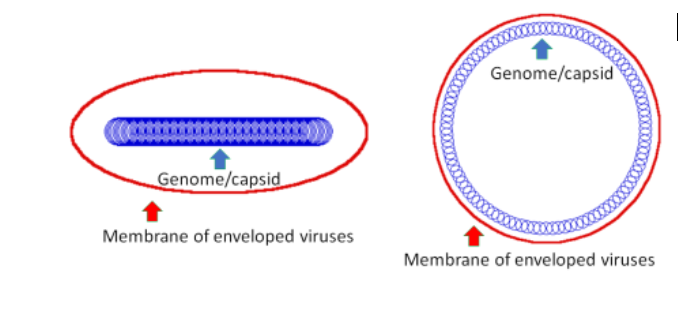
\includegraphics[width=0.5\textwidth,height=3.7cm]{monkeypox.png}}  % Adjust width or height as needed
  \caption{Preliminary 2D model studies to
investigate the effect of the geometry of a
genome on the shape of a virus. A rod-like
genome induces an elliptic shape whereas a
circular genome leads to a circular shape.}
\end{figure}




\subsection*{IV.Projected timeline}

Months 0-3: Fine-tune the continuum membrane model.\\
Months 4-6: Investigate competition among different membrane shapes.\\
Months 7-9: Study chain model and crowding effect\\
Months 10-12:Expand the developed models from 2D to 3D.\\









\newpage

\end{flushleft}
\bibliographystyle{unsrt}
\bibliography {references}  

\end{document}




